\section{Conceptos previos}
En este apartado se describe la arquitectura de VMware Cloud Foundation y como estructura sus componentes\footnote{Se describen solo aquellos componentes que se utilizarán en el despliegue de Cloud Foundation.} internamente.

%%%%%%%%%%%%%%%%%%%%%%%%%%%%%%
\iffalse
En este apartado se explican aquellos conceptos de VMware Cloud Foundation necesarios para entender su funcionamiento, configuración y requisitos de la infraestructura previos al despliegue del servicio.
\fi
%%%%%%%%%%%%%%%%%%%%%%%%%%%%%%%%


%% Workload Ddomains %&%&%%%%
%%%%%%%%%%%%%%%%%%%%%%%%%%%%
\subsection{Workload Domain}
Un \textit{workload domain} consiste en una instancia lógica de un SDDC que abarca todos o parte de los recursos de uno o más clusters, cuya función es aislar el flujo de trabajo de un usuario, aplicación o un determinado tipo de tareas. Cada \textit{workload domain} se extiende sobre varios hosts y contiene su propia instancia de vCenter Server, vSAN y NSX, lo cual permite establecer políticas de control únicas para todos los \textit{workload domains} y específicas para cada uno de ellos a la vez que se simplifica la complejidad de la infraestructura. Existen \underline{tres tipos} de \textit{workload domains} que permiten aislar las tareas de gestión de la infraestructura del resto de flujos de trabajo. 

%% MANAGEMENT DOMAIN
\subsubsection{Management Domain}
\label{subsubsec:domainManagement}
Este \textit{workload domain} se crea y configura automáticamente durante el proceso de despliegue de una instancia de VMware Cloud Foundation. Su función es gestión de todos los componentes de VMware Cloud Foundation, de toda la infraestructura y del resto de \textit{workload domains} existentes en el entorno a tráves de políticas establecidas desde un único punto. Los componentes dedicados a este \textit{workload domain} son SDDC Manager, vCenter Server, una instancia de NSX Manager, tres instancias de NSX Controller, dos instancias de Platform Services Controller y tres instancias de vRealize Log Insight \cite{sddcComponents} [Fig. \ref{fig:componentsMNGDomain}].\\
Cuando se \underline{despliega \textit{management domain} se crean y configuran} de forma automatizada por SDDC Manager las siguientes máquinas virtuales (VM) de cada componente de Cloud Foundation\footnote{Las características de cada máquina virtual se refieren a los requisitos mínimos}:
\begin{itemize}
    \item Una VM de \textbf{SDDC Manager}: 4 vCPU, 16 GB de memoria, 800 GB de almacenamiento.
    \item Una VM de \textbf{vCenter Server}: 4 vCPU, 16 GB de memoria, 290 GB de almacenamiento.
    \item Dos instancias de \textbf{Platform Services Controller} (cada una): 2 vCPU, 4 GB de memoria, 60 GB de almacenamiento.
    \item Una VM de \textbf{NSX Manager}: 4 vCPU, 16 GB de memoria, 60 GB de almacenamiento.
    \item Tres VM de \textbf{NSX Controller} (cada una): 4 vCPU, 4 GB de memoria, 28 GB de almacenamiento.
    \item Tres VM de \textbf{vRealize Log Insight}: 4 vCPU, 8 GB de memoria, 250 GB de almacenamiento.
\end{itemize}

Para desplegar un \textit{management domain} se requieren las siguientes \underline{capacidades mínimas} en la infraestructura \cite{WDminRequierements}:
\begin{itemize}
    \item \textbf{Hosts}: 4
    \item \textbf{CPU} por host: Dual-socket con 8 cores por socket, en sistemas All-Flash.
    \item \textbf{Memoria} total: 192 GB
    \item \textbf{Almacenamiento} por host: 16 GB para el dispositivo de arranque, un NVMe o SSD para la capa de caché, dos SSD o HDD para la capa de capacidad\footnote{En total se requieren 800 GB para este \textit{workload domain}.}.
    \item \textbf{NICs} por host: Dos NICs de al menos 10 GbE y, opcionalmente un NIC 1GbE BMC.
\end{itemize}

\begin{figure}[h!]
  \centering
  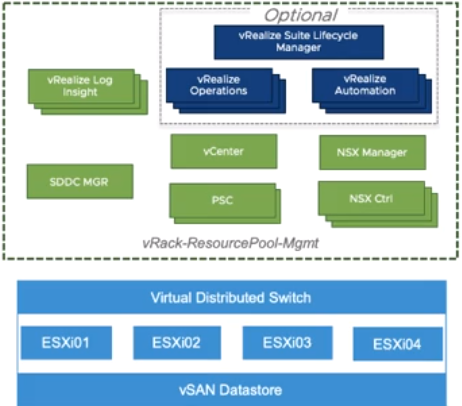
\includegraphics[width=0.5\textwidth]{imaxes/conceptosPrevios/componentsMANAGEDomain.png}
  \caption{Componentes de \textit{management domain}}
  \label{fig:componentsMNGDomain}
\end{figure}
\FloatBarrier 


%% VIRTUAL INF. DOMAIN
\begin{subsubsection}{Virtual Infrastructure Domain (VI) y Virtual Desktop Infrastructure Domain (VDI)}
\label{subsubsec:domainVI}
Este tipo de \textit{workload domain} se crea manualmente y bajo demanda desde \textit{management domain} para dar servicio a las necesidades de cada usuario o para crear diferentes entornos con finalidades distintas. Su configuración de hardware y lógica se especifican durante su proceso de creación, permitiendo indicar la cantidad de hosts, cantidad de almacenamiento, configuración de la red y políticas de rendimiento y disponibilidad, todo para satisfacer las necesidades del tipo de tareas para las que se crea. El acceso a un \textit{VI domain} se realiza a través de vSphere Client donde el administrador puede gestionar todos los recursos asociados con ese \textit{workload domain}. Cada \textit{virtual infrastructure domain} cuenta con sus propios vCenter Server y un NSX Manager dedicados, que se ejecutan desde el \textit{management domain} de la infraestructura, y \textit{datastore} vSAN dedicado. La diferencia entre un \textit{virtual infrastructure domain} y \textit{virtual desktop infrastructure domain} es que el segundo incorpora el producto VMware Horizon View que, resumiendo, permite desplegar escritorios virtuales. Con cada nuevo \textit{virtual infrastructure domain} se crea un nuevo cluster vSphere en la infraestructura que agrupa todos los recursos que tiene asignados.\\
Cuando se \underline{despliega un \textit{virtual infrastructure domain} se crean y configuran} de forma automatizada por el componente SDDC Manager las siguientes máquinas virtuales (VM) de cada componente de VMware Cloud Foundation\footnote{Las características de cada máquina virtual se refieren a los requisitos mínimos} \cite{sddcComponents} [Fig. \ref{fig:compoVIdomain}]:
\begin{itemize}
    \item Una VM de \textbf{vCenter Server} en Management Domain: 8 vCPU, 24 GB de memoria, 500 GB de almacenamiento.
    \item Una VM de \textbf{NSX Manager} en Management Domain: 4 vCPU, 16 GB de memoria, 60 GB de almacenamiento.
    \item Tres VM de \textbf{NSX Controller} en el VI Domain creado (cada una):  4 vCPU, 4 GB de memoria, 28 GB de almacenamiento.
\end{itemize}

Por cada \textit{virtual infraestructure domain} que se despliega en la infraestructura, se requieren las siguientes capacidades mínimas\cite{WDminRequierements}:
\begin{itemize}
    \item \textbf{Hosts}: 3
    \item \textbf{CPU}, \textbf{Memoria} y \textbf{Almacenamiento}: depende de los requisitos de las tareas que se vayan a desarrollar en este \textit{workload domain}.
    \item \textbf{NICs} por servidor: Dos NICs de al menos 10 GbE y, opcionalmente un NIC 1 GbE BMC.
\end{itemize}


\end{subsubsection}

\begin{figure}[h!]
  \centering
  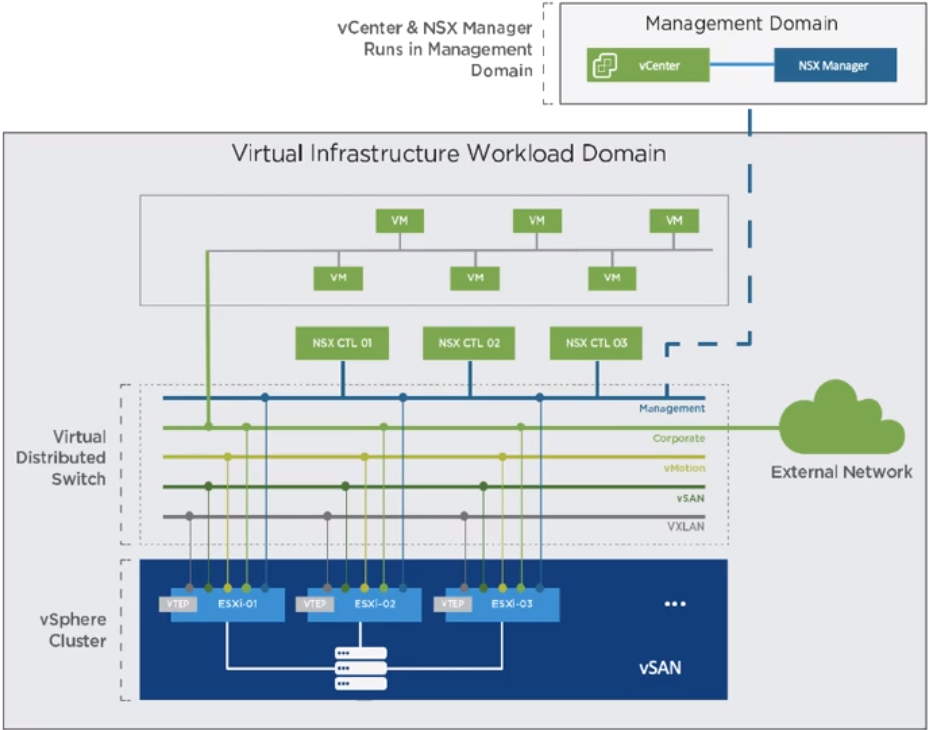
\includegraphics[width=0.5\textwidth]{imaxes/conceptosPrevios/networkArcVIDomain.png}
  \caption{Componentes de \textit{virtual infrastructure domain}.}
  \label{fig:compoVIdomain}
\end{figure}
\FloatBarrier

%&%%%%%%%%%%%%%%%%%%%%%%%%%%%%%%%%%%%%%%%%%%%%%%%%%%%%%%%%
%% ARQUITECTURA



\subsection{Arquitectura}
La arquitectura de VMware Cloud Foundation tiene dos posibles modelos de despliegue dependiendo del número de hosts sobre los que se despliega VMware Cloud Foundation.

%% ESTANDAR
\subsubsection{Modelo estándar}
Este modelo está pensado para desplegar VMware Cloud Foundation en entornos de tamaño medio/grande con un mínimo de siete hosts. Está formado por un \textit{management domain} que se despliega en cuatro de los hosts y contiene todos los componentes de gestión de toda la infraestructura, desde este \textit{workload domain} se administra la infraestructura del SDDC y cada \textit{virtual infrastructure domain} existente. Además, este modelo contiene al menos un \textit{virtual infrastructure domain}, creado bajo demanda y con capacidades establecidas según su finalidad que posteriormente se pueden pueden modificar, se despliega sobre al menos tres hosts. Cada \textit{virtual infrastructure domain} requiere tres hosts adicionales, es decir, un host solo puede pertenecer a un único \textit{workload domain}. El máximo número de \textit{virtual infrastructure domains} que se pueden desplegar en una instacia de VMware Cloud Foundation es 14.

\begin{figure}[h!]
  \centering
  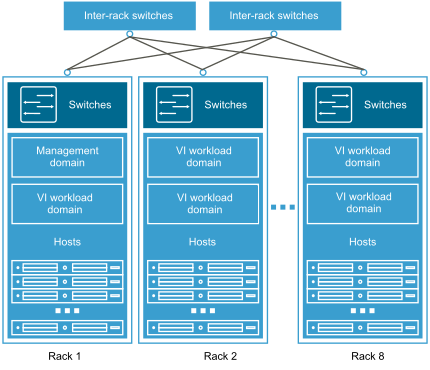
\includegraphics[width=0.6\textwidth]{imaxes/conceptosPrevios/arquitect_standarCF.png}
  \caption{Esquema del modelo de arquitectura estándar.}
  \label{fig:modelostandard}
\end{figure}

\begin{figure}[h!]
  \centering
  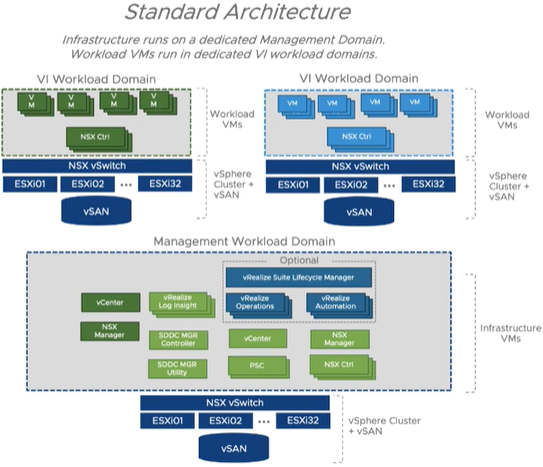
\includegraphics[width=0.6\textwidth]{imaxes/conceptosPrevios/standardArch.png}
  \caption{Estructura de los componentes en una arquitectura estándar.}
  \label{fig:standardarch}
\end{figure}
\FloatBarrier
%%%%%%%%%%%%%%%%%%%%%
%%  CONSOLIDADO
\subsubsection{Modelo consolidado}
Este modelo está pensado para desplegar VMware Cloud Foundation en entornos de tamaño pequeño, normalmente cuando hay menos de siete hosts, aunque se puede también se puede utilizar sobre entornos más grandes de hasta 64 hosts. En este modelo los flujos de trabajo que corresponden al \textit{virtual infrastructure domain} y al \textit{management domain} en el despliegue estándar, están colocados dentro de un mismo \textit{workload domain} en un único cluster pero aislados gracias a que cada uno se coloca dentro de un \textit{resource pool}, es decir, solo existe un cluster con varios \textit{resource pool}. Un \textit{resource pool} es una carcaterística de VMware vSphere que permite abstraer un conjunto de recursos de un cluster estableciendo unos límites de capacidad que puede usar \cite{resourcePool}. Este modelo se puede convertir en un modelo estándar creando un \textit{virtual infrastructure domain}.[Fig. \ref{fig:modeloconsolidated}].

\begin{figure}[h!]
  \centering
  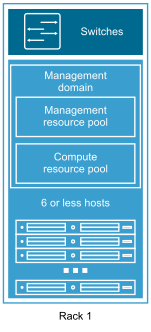
\includegraphics[width=0.25\textwidth]{imaxes/conceptosPrevios/modelConsolidated.png}
  \caption{Esquema del modelo de arquitectura consolidado.}
  \label{fig:modeloconsolidated}
\end{figure}

\begin{figure}[h!]
  \centering
  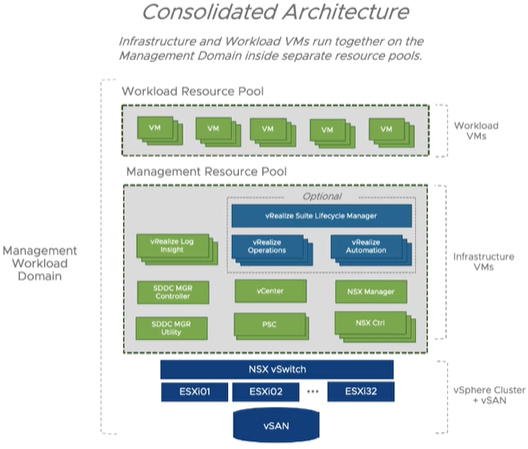
\includegraphics[width=0.85\textwidth]{imaxes/conceptosPrevios/consolidatedArch.png}
  \caption{Estructura de los componentes de una arquitectura consolidado.}
  \label{fig:consolidatedArch}
\end{figure}
\FloatBarrier


\section{Requisitos y diseño de la infraestructura y arquitectura}

Teniendo en cuenta las capacidades físicas de la infraestructura, se ha elegido el modelo consolidado para el despliegue de VMware Cloud Foundation sobre la infraestructura. 
La principal razón por las que se escoge este modelo es por el número de hosts ESXi.\\
En los siguientes apartados se describen la arquitectura que se genera y la infraestructura requerida en cada capa.

%%%% DISEÑO ARQUI. FÍSICA %%%%%
\begin{subsection}{Arquitectura e Infraestructura Físicas \cite{CFfisInfraestuctura}}
En este apartado se describen las principales características que tiene el entorno físico de un SDDC construído con VMware Cloud Foundation.

\subsubsection{Clusters, zonas de disponibilidad y regiones}
Un SDDC puede estar formado por uno o más clusters de distintos tipos. En el  \underline{modelo consolidado} la infraestructura está formada por un único cluster que incluye los servicios de gestión de VMware Cloud Foundation VMware vCenter Server, vSphere Update Manager, VMware NSX Manager, VMware NSX Controller y VMware vRealize Log Insight, los servicios de red necesarios para establecer conectividad en el entorno y las máquinas virtuales que los usuarios crean cuando aprovisionan sus recursos. Se aplican las mismas políticas de alta disponibilidad y gestión del ciclo de vida al flujo de trabajo de gestión del SDDC y al flujo de trabajo del usuario. En el \underline{modelo estándar} los distintos \textit{workload domain} se dividen en clusters que pueden ser de tres tipos:
    \begin{itemize}
        \item \textbf{Management Cluster}: se crea durante el despliegue de VMware Cloud Foundation y contiene el \textit{management domain}, desde aquí se gestiona el SDDC. Contiene los servicios de gestión mecionados anteriormente.
        \item \textbf{Shared Edge and Compute Cluster}: es el primer cluster que se crea dentro de un \textit{virtual infrastructure domain} ya que puede haber más de un cluster. Este cluster contiene los servicios de red NSX del \textit{workload domain} y también puede contener el flujo de trabajo de los usuarios.
        \item \textbf{Compute Cluster}: cluster adicional que se crea dentro de un \textit{virtual infraestructure domain}. Contiene el flujo de trabajo de los usuarios.
    \end{itemize}
Un SDDC puede estar distribuído en una o más \textit{Availability Zone} (AZ). Estas son zonas aisladas con infraestructuras independientes que evitan la propagación de fallos de hosts individuales a través de toda la infraestructura, cuantas más \textit{AZ} existan mayor disponibilidad tendrá el servicio. La latencia entre dos \textit{AZ} debe ser de 5 ms como máximo y la conexión de al menos 10 Gbit. Una \textit{Region} agrupa una o más \textit{AZ}s, con esto se da solución a la recuperación del servicio ante desastres. La latencia entre dos \textit{Region}s debe ser de 100 ms como máximo. El \underline{modelo consolidado} solo da soporte a una \textit{Region} con una \textit{AZ}, mientras que el \underline{modelo estándar} puede soportar múltiples \textit{Region}s con múltiples \textit{AZ}s.

%%%%%%%%%%%%%%%%%%%%%%%%%%%%%%%%%%%%%%%%%%%%
%%%%%%%%%%%%%%%%%%%%%%%%%%%%%%%%%%%%%%%%%%%%
%%%%%%%%%%%%%%%%%%%%%%%%%%%%%%%%%%%%%%%%%%%%
\iffalse
Un SDDC puede estar \underline{formado por múltiples clusters} que pueden ser de diferentes tipos con diferentes propósitos. Un cluster puede ocupar uno o más \textit{racks} dependiendo del nivel de escalabilidad que se requiera. Según su función, cada \textit{workload domain} se puede colocar en un cluster diferente para gestionar la alta disponibilidad y el ciclo de vida según sus necesidades. Un \underline{cluster puede ser de varios tipos}:
\begin{itemize}
    \item \textbf{Management Cluster}: Es aquel que contiene el \textit{management domain}, por lo tanto contiene las máquinas virtuales de los componentes que gestionan el SDDC. A este cluster solo deben acceder los administradores de la infraestructura.
    \item \textbf{Shared Edge y Compute Cluster}: contiene el \textit{virtual infrastructure domain} con las máquinas virtuales de los usuarios y, además, incorpora servicios de NSX necesarios para comunicarse con redes externas y con otros \textit{workload domains}.
    \item \textbf{Compute Cluster}: solo contiene el \textit{virtual infrastructure domain} con las máquinas virtuales de los usuarios.
    \item \textbf{External Storage}: se centra en proveer almacenamiento de tipo NFS, iSCSI o Fiber Channel.
\end{itemize}

Un SDDC puede estar distribuído en una o más \underline{zonas de disponibilidad}. Estas son zonas aisladas que evitan la propagación de fallos de hosts individuales a través de toda la infraestructura, así, se puede entregar mayor disponibilidad de los recursos y servicios. A su vez, varias \underline{zonas de disponibilidad} se pueden agrupar en una \underline{región}, estos entornos separados por grandes distancias que permiten tener recuperación ante desastres [Fig. \ref{fig:AVRegiones}].\\

\begin{figure}[h!]
  \centering
  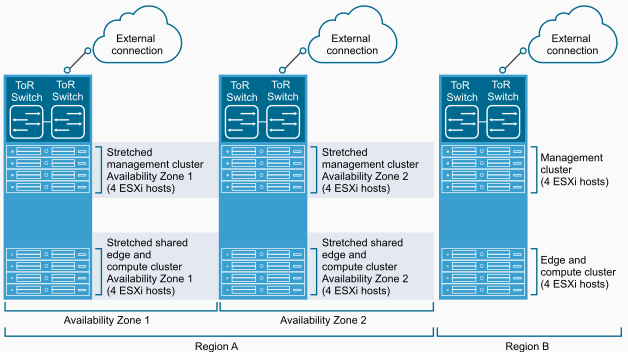
\includegraphics[width=0.95\textwidth]{imaxes/conceptosPrevios/zonasDispRegiones.png}
  \caption{Una región contiene al menos una zona de disponibilidad.}
  \label{fig:AVRegiones}
\end{figure}
\fi
%%%%%%%%%%%%%%%%%%%%%%%%%%%%%%%%%%%%%%%%%%%%%
%%%%%%%%%%%%%%%%%%%%%%%%%%%%%%%%%%%%%%%%%%%%%
%%%%%%%%%%%%%%%%%%%%%%%%%%%%%%%%%%%%%%%%%%%%%

\FloatBarrier

\subsubsection{Red física}
La topología de red en la capa física del SDDC de VMware Cloud Foundation se puede implementar mediante servicios de \underline{transporte} en la capa 2 o en la capa 3. El \underline{diseño en la capa 2} implica que la topología de la red incluya los dispositivos de capa 2 (\textit{Top of Rack Switches}) y los dispositivos de la capa 3 (routers, switches) [Fig. \ref{fig:transportlayer2}], por lo tanto las VLANs que se definan se deben implementar en la capa 2 y en la capa 3. Esto puede provocar problemas al aumentar el tamaño de la red ya que el número de VLANs disponible es más limitado, y problemas de compatibilidad ya que es posible que los dispositivos físicos tengan que ser del mismo proveedor. El \underline{diseño en la capa 3} implica que la topología de la red solo incluye a los dispositivos de capa 3 [Fig. \ref{fig:transportlayer3}]. Esto permite limitar la definición de VLANs a esa capa y el uso de enrutamiento dinámico con protocolos OSPF o BGP entre la capa 2 y 3. Así se consigue una mayor libertad a la hora de seleccionar los dispositivos físicos de red y que su configuración es más sencilla.
\begin{figure}[h!]
  \centering
  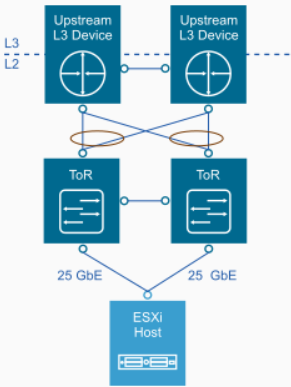
\includegraphics[width=0.3\textwidth]{imaxes/conceptosPrevios/transportlayer2.png}
  \caption{Límite de las capas 2 y 3 cuando la topología se implementa con dispositivos de capa 2.}
  \label{fig:transportlayer2}
\end{figure}
\FloatBarrier
\begin{figure}[h!]
  \centering
  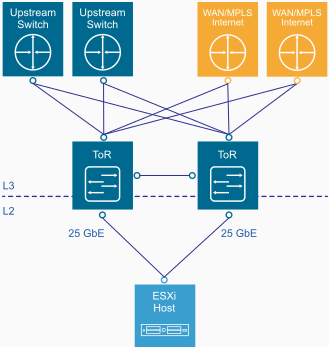
\includegraphics[width=0.3\textwidth]{imaxes/conceptosPrevios/transportNetLayer3.png}
  \caption{Límite de las capas 2 y 3 cuando la topología se implementa con dispositivos de capa 3.}
  \label{fig:transportlayer3}
\end{figure}
\FloatBarrier

\iffalse
n los componentes de VMware, o en la capa tres, para usar dispositivos de transporte lógico. Cada tipo de configuración tiene sus ventajas y desventajas, pero la configuración más común en este tipo de entornos es usar el transporte de red sobre la capa tres ya que da más libertad a la hora de gestionar y configurar los recursos físicos de red.\\
\fi

Como VMware Cloud Foundation abstrae la red física en una red virtual, la red física debe cumplir ciertos requisitos para que la red virtualizada sea robusta. Esta se debe mantener simple con configuraciones comunes en todos los switches, uso de VLANs y uso de enrutamiento dinámico, también debe ser escalable en cuanto a cantidad de hosts, ancho de banda y cantidad de rutas redundantes. Además, se debe tener en cuenta que cada tipo de tráfico tiene características diferentes, como por ejemplo el tráfico dedicado al almacenamiento a través de IP que suele usar mayor ancho de banda, por ello es necesario distinguir cada tipo de tráfico con protocolos \textit{Quality of Service} (QoS). El marcado de cada tipo de tráfico se realiza en el hipervisor ESXi a través de un vSphere Distributed Switch que soporta QoS tanto en la capa 2 como en la capa 3. En la capa 2 se utiliza  un campo de tres bits llamado \textit{Class of Service} que representa la prioridad del \textit{frame} con un valor de cero a siete, presente en la cabecera Ethernet cuando se utiliza etiquetado VLAN, mientras que en la capa 3 se utiliza un campo de 6 bits en la cabecera IP llamado \textit{Differentiated Services Code Point}, perteneciente al protocolo \textit{DiffServ}, para clasificar cada paquete. Los \underline{principales componentes que se deben configurar} para dar conectividad entre los servidores son los siguientes:
\begin{itemize}
    \item \textbf{Top of Rack Physical Switches} (TOR): es un switch al que se conectan los hosts de un rack para tener conectividad con el resto de la infraestructura. Se recomienda que un host esté conectado a dos switches TOR y que estos se configuren de forma redundante para proveer alta disponibilidad y tolerancia a fallos de alguna de las conexiones. Cada switch TOR se conecta a otro par de switches que establece conexión entre todos los racks.
    
    Los puertos del switch TOR que se conectan a los hosts deben estar configurados como puertos troncales de VLAN para que acepte todas las VLANs usadas por el host, se debe proveer servicio DHCP a cada VLAN usada y configurar los puertos para que acepten \textit{jumbo frames}. El marcado QoS del tráfico que realiza cada host ESXi debe ser aceptado y no puede ser modificado una vez abandona el host. \iffalse Además, se deben configurar todas las VLANs y subredes que se utilizarán en la infraestructura de VMware Cloud Foundation.\fi  
    
    \underline{Otros protocolos que se deben configura}r en los puertos que se conectan con los hosts son:
    \begin{itemize}
        \item \emph{Spanning Tree Protocol} (STP): protocolo que se encarga de gestionar las rutas de la red que son redundantes.
        \item \emph{Trunking}: configurar cada enlace troncal con las VLANs que van a transmitir tráfico a través de él. Se debe establecer como VLAN nativa, aquella utilizada para transmitir el tráfico que no tiene etiqueta, VLAN de la red \textit{management}.
        \item \emph{MTU}: configurar el MTU de cada VLAN para el transporte de paquetes \textit{jumbo frames}. Este valor será el que se use para configurar los hosts ESXi. Se recomienda establecerlo en 9000 bytes.
        \item \emph{Multicast}: configurar el protocolo IGMP en cada switch TOR como enrutador (busca activamente que VLANs pertenecen a un grupo Multicast) y cada VLAN como miembros de IGMP (los hosts que forman parte del grupo indican su pertenencia a un grupo multicast de forma activa).
    \end{itemize}
    

    
    \iffalse
    \item \textbf{Conectividad entre Regiones}: 
    \item \textbf{Conectividad entre Zonas de dispobilidad}:
    \fi
\end{itemize}

Los siguientes servicios usados por los componentes de VMware Cloud Foundation se deben configurar sobre la red física de la infraestructura para el correcto funcionamiento del SDDC\cite{CFexternalServices}:
\begin{itemize}
    \item \textbf{Servidor DNS}: se utiliza para obtener los nombres y direcciones de todas las máquinas virtuales que se creen, tanto en sentido \textit{fordward} (obtener una dirección IP a partir de un nombre) como en sentido \textit{reverse} (obtener un nombre a partir de una dirección IP). Además, este servicio debe ser configurado antes de realizar el despliegue de VMware Cloud Foundation. Este servicio es utilizado por el componente Platform Services Controller, vCenter Server, NSX Manager y vRealize Log Insight.
    
    \item \textbf{Servidor DHCP}: permite asignar direcciones IP de forma dinámica a los puertos \textit{vmkernel} de cada host ESXi. Este debe ser accesible desde cada VXLAN de VMware NSX y es necesario establecer previamente las redes que se van a usar en VMware Cloud Foundation. Este servicio debe estar disponible antes de comenzar el despliegue del SDDC ya que es necesaria la asignación dinámica de IPs.
    
    \item \textbf{Servidor NTP}: requerido por todos los componentes de VMware Cloud Foundation para mantener sus horas sincronizadas. Este servicio debe estar disponible en la infraestructura y configurado en cada host ESXi antes del despliegue de VMware Cloud Foundation, y debe ser alcanzable desde la red de \textit{management} y de vRealize. La derencia de tiempo entre los componentes de la infraestructura no debe ser mayor de cinco minutos.
    
    \item \textbf{Router}: debe existir enrutamiento dinámico en la red desde la capa 3. Es requerido por NSX para establecer comunicación con los ESG. Este servicio debe estar configurado antes del comenzar enl despliegue de VMware Cloud Foundation. 
\end{itemize}

\subsubsection{Host ESXi\cite{WDminRequierements}}
Los hosts ESXi que se desplieguen en un cluster deben tener características físicas idénticas para hacer la infraestructura más manejable,  incluyendo la configuración de almacenamiento y red. Para desplegar VMware Cloud Foundation se requiere:
\begin{itemize}
    \item  Dos interfaces de red (NIC) de la misma velocidad que deben estar conectadas a la VLAN troncal de dos switches TOR. Configurando \textit{NIC teaming} en VMware Sphere Distributed Switch se consigue que el tráfico se distribuya por las interfaces de red disponibles de forma óptima y que exista tolerancia a fallos.
    \item Todas las conexiones físicas del host deben tener al menos una velocidad igual a 10 Gbit.
    \item Cada host debe tener al menos 192 GB de memoria RAM, de esa cantidad, 176 GB de memoria RAM son requeridos por las máquinas virtuales que gestionan el SDDC.
    \item Un disco de arranque con un tamaño mínimo de 16 GB.
\end{itemize}

\subsubsection{Almacenamiento físico}
VMware Cloud Foundation utiliza VMware vSAN para proveer el almacenamiento de un SDDC. Para desplegar VMware Cloud Foundation, VMware vSAN requiere las siguientes características:
\begin{itemize}
    \item Mínimo de tres hosts con recursos de almacenamiento.
    \item Determinar qué configuración de vSAN se va a utilizar, \textit{All-Flash} o \textit{Hybrid}. Se recomienda la solución \textit{All-Flash} ya que ofrece mayor rendimiento.
    \item Para cada host con recursos de almacenamiento se debe cumplir que el disco de caché tenga un 10\% de la capacidad del almacenamiento persistente del grupo de discos, tener un mínimo de dos discos en la capa de capacidad, un controlador RAID y configurar habilitar vSphere High Availability  para apagar las máquinas virtuales de un host cuando este se encuentre aislado. El controlador RAID debe tener la característica \textit{pass-through} la cual permite que VMware vSAN muestre como discos individuales cada disco duro de un grupo de discos, esto facilita la gestión de cada disco y que se puedan realizar sustituciones sin detener el servicio.
    \item La capacidad mínima de almacenamiento disponible para el modelo consolidado es de 800 GB. 
\end{itemize}

\end{subsection}



%%%%%DISEÑO ARQ. VIRTUAL
\begin{subsection}{Arquitectura e Infraestructura Virtuales\cite{CFVirtInfraes}}
%%%%%%%%%%%%%%%%%%%%%%%%%%%%%%%%%%%%%%%%%%%%%
%%%%%%%%%%%%%%%%%%%%%%%%%%%%%%%%%%%%%%%%%%%%%
%%%%%%%%%%%%%%%%%%%%%%%%%%%%%%%%%%%%%%%%%%%%%
\iffalse
La infraestructura virtual de un SDDC puede estar formada por una o más regiones, cada una tiene su propio \textit{management domain} que contiene el \textit{management cluster}, y un \textit{virtual infrastructure domain} que contiene el \textit{shared cluster} y un \textit{compute cluster}.
\fi
%%%%%%%%%%%%%%%%%%%%%%%%%%%%%%%%%%%%%%%%%%%%%
%%%%%%%%%%%%%%%%%%%%%%%%%%%%%%%%%%%%%%%%%%%%%
%%%%%%%%%%%%%%%%%%%%%%%%%%%%%%%%%%%%%%%%%%%%%

Esta capa virtual provee infraestructura de almacenamiento, red y cómputo definida por software a través de servicios. En el modelo de despliegue consolidado de VMware Cloud Foundation, todos sus servicios y componentes se encuentran dentro de un mismo cluster (solo una AZ) dentro de la infraestructura, mientras que en el modelo estándar los servicios y componentes de gestión de la infraestructura están situados en clusters distintos (pueden estar en AZ distintintas), todos sus componentes se encuentran agrupados en un mismo cluster.



\subsubsection{Diseño de VMware vCenter Server}
El componente VMware vCenter Server es el punto de acceso y de control de todas las máquinas virtuales y servicios localizados en los hosts ESXi que forman parte de su dominio. En VMware Cloud Foundation se utiliza una instancia de VMware vCenter Server para controlar un \textit{workload domain}, por lo tanto en este modelo existen al menos dos instancias. Esto permite aislar el flujo de trabajo del \textit{management domain} de cada \textit{virtual infrastructure domain}, simplificar la escalabilidad del SDDC y el uso de un NSX Manager por cada \textit{workload domain} para aislar su red. Además, VMware vCenter Server requiere los servicios localizados en el componente PSC que se puede desplegar de dos formas, embebido en la misma instancia de vCenter Server o en una máquina virtual externa a vCenter Server. La segunda opción permite compartir la misma instancia de PSC entre varias instancias de vCenter Server. En el modelo consolidado solo se despliega una instancia de VMware vCenter Sever.\\
Para ambos modelos de despliegue se recomienda situar las instancias de PSC que se creen, en un entorno externo a VMware vCenter Server con el fin de facilitar la creación de nuevos \textit{workload domains}.


%%%%%%%%%%%%%%%%%%%%%%%%%%%%%%%%%%%%%%%%%%%%%%%%%%%%%%%%%%%%%
%%%%%%%%%%%%%%%%%%%%%%%%%%%%%%%%%%%%%%%%%%%%%%%%%%%%%%%%%%%%%
%%%%%%%%%%%%%%%%%%%%%%%%%%%%%%%%%%%%%%%%%%%%%%%%%%%%%%%%%%%%%
%%%%%%%%%%%%%%%%%%%%%%%%%%%%%%%%%%%%%%%%%%%%%%%%%%
%%%%%%%%%%%%%%%%%%%%%%%%%%%%%%%%%%%%%%%%%%%%%%%%%%%%%%%%%%%%%
%%%%%%%%%%%%%%%%%%%%%%%%%%%%%%%%%%%%%%%%%%%%%%%%%%%%%%%%%%%%%

\subsubsection{Diseño de cada cluster VMware vSphere}
En un SDDC se pueden crear varios clusters vSphere con distintas finalidades, según la cantidad de hosts ESXi, la capacidad de cada uno y del uso que se va a realizar de cada cluster. Además, dentro de la configuración de un cluster hay que considerar como se va a configurar el componente vSphere High Availability para establecer una política de reserva de recursos para restaurar recursos en caso de que un host esté inactivo por algún fallo.\\

En el modelo consolidado se debe crear un único cluster con un mínimo de cuatro hosts ESXi ya que uno de los hosts se utiliza para asegurar la disponibilidad del almacenamiento vSAN cuando hay algún host inactivo. Este modelo proporciona capacidad de un único fallo por cluster.

%%%%%%%%%%%%%%%%%%%%%%%%%%%%%%%%%%%%%%%%%%%%
\subsubsection{Red Virtual}
En esta sección se describe como VMware Cloud Foundation abstrae la red física en un conjunto de recursos virtuales de red, utilizando los servicios de VMware NSX para crear una capa virtual independiente de la infraestructura física.
Los componentes de VMware NSX se distribuyen de forma diferente dependiendo de si se utiliza el modelo consolidado o el estándar. En el modelo consolidado, la instancia de NSX Manager, las instancias de NSX Controller y cada NSX ESG y NSX DLR están situados en el mismo cluster. En el modelo estándar, cada AZ contiene en el \textit{management cluster} las instancias de NSX Manager para cada \textit{workload domain}, las instancias de NSX Controller para el \textit{management domain} y las máquinas virtuales de NSX ESG y DLR Control para el \textit{management domain}, el cluster \textit{shared edge and compute} contiene las instancias de NSX Controller de cada \textit{virtual infrastructure domain} y las máquinas virtuales de NSX ESG y DLR Control de cada \textit{virtual infraestructure domain}. En ambos modelos las instancias de NSX Manager proveen alta disponibilidad gracias al servicio vSphere HA, los componentes del \textit{data plane} permanencen activos aunque el \textit{control} y \textit{management} \textit{planes} estén fuera de servicio. Las instancias de NSX Controller se distribuyen entre todos los hosts ESXi por el servicio vSphere DRS.
 Esto se hace posible principalmente gracias a NSX Logical Switch y a VXLAN.\\
A continuación se exponen varios aspectos generales que se deben tener en cuenta antes de diseñar la configuración de la red virtual:
\begin{itemize}
    \item Segmentar los diferentes tipos de tráfico para mejorar la eficiencia de la red y la seguridad. Así se puede ajustar las características de cada red, como el ancho de banda o la latencia, a las necesidades de cada servicio.
    \item Utilizar un único vSphere Distributed Switch por cluster con las distintas redes dedicadas a cada servicio y con diferentes VLANs. La configuración de VLANs debe coincidir con la establecida en la capa física.
    \item Mejorar el rendimiento usando NICs de tipo VMXNET3 en las máquinas virtuales.
    \item Las NICs físicas de cada host ESXi conectadas a un mismo vSphere Distributed Switch deben estar conectadas también a la misma red física.
    \item Aquellas redes que se dedican a servicios de la infraestructura deben estar configuradas con puertos tipo \textit{vmkernel}.
\end{itemize}

Para segmentar la red se configura en un vSphere Distributed Switch una VLAN por cada tipo de tráfico que genera VMware vSphere\footnote{Las VLANs descritas se corresponden con el \textit{management} cluster de la arquitectura estándar y con el cluster de la arquitectura consolidada. El resto de clusters del modelo estándar tienen solo las VLANs de los servicios que hay en ellos.}:
    \begin{itemize}
        \item \textbf{Management}: esta VLAN comunica todos los hosts ESXi y por ella se transmite el tráfico enviado entre servicios de VMware Cloud Foundation. Por defecto está configurada en un \textit{vmkernel} con MTU igual a 1500
        \item \textbf{vMotion}: por esta VLAN circula el tráfico del componente vSphere vMotion para realizar las migraciones de máquinas virtuales de un host a otro. Se configura en un \textit{vmkernel} con MTU igual a 9000.
        \item \textbf{vSAN}: a través de esta VLAN los hosts acceden al servicio de almacenamiento mediante dirección IP. Se configura en un \textit{vmkernel} con MTU igual a 9000.
        \item \textbf{VM Network}: por esta VLAN circula el tráfico de las aplicaciones y máquinas virtuales de los usuarios. Se asigna a un \textit{vmportgroup}.
    \end{itemize}
Desde el vSphere Distributed Switch se configuran de forma centralizada todas las VLANs existentes en un cluster. Permite establecer las siguientes características:
\begin{itemize}
    \item \textit{Network I/O Control}: permite establecer un nivel de prioridad a cada VLAN según el servicio que la utiliza sea más o menos crítico. Esto se realiza estableciendo limites de ancho de banda, políticas de balanceo de carga y reserva de recursos para una funcionalidad específica de vSphere.
    \item \textit{NIC Teaming}: permite aumentar el ancho de banda de la red, balancear la carga del tráfico y reducir el riesgo de fallos. Para poder aplicar esta configuración el host ESXi debe tener conectadas dos NICs al Distributed Switch que físicamente se conectan a dos switches diferentes.
\end{itemize}

Las redes VLAN creadas funcionan sobre el protocolo IP de la red física gracias a \textit{Virtual Extensible LAN} (VXLAN). Este protocolo permite enviar un tráfico de capa de datos (capa 2) encapsulado en \textit{frames} de capa de red (capa 3) existente en la infraestructura de red física creando lo que se llama una \textit{transport zone}, la cual delimita el alcance de una VXLAN. Cada VXLAN está identificada por su \textit{VXLAN Network Identifier} (VNI), un número de 24 bits. La encapsulación y transmisión del tráfico a la red es realizada por un \textit{VXLAN Tunnel End Point} (VTEP) situado en cada host ESXi en un puerto \textit{vmkernel}
dentro de vSphere Distributed Switch, cada uno tiene una IP asignada. Cada \textit{transport zone} se puede extender por varios vDS, el acceso a ella lo proporciona un Logical Switch configurado epecificamente para una  \textit{transport zone} [Fig. \ref{fig:trasnportZoneSpan}]. En un mismo vDS se puede tener acceso a varias \textit{transport zone}. 

\begin{figure}[h!]
  \centering
  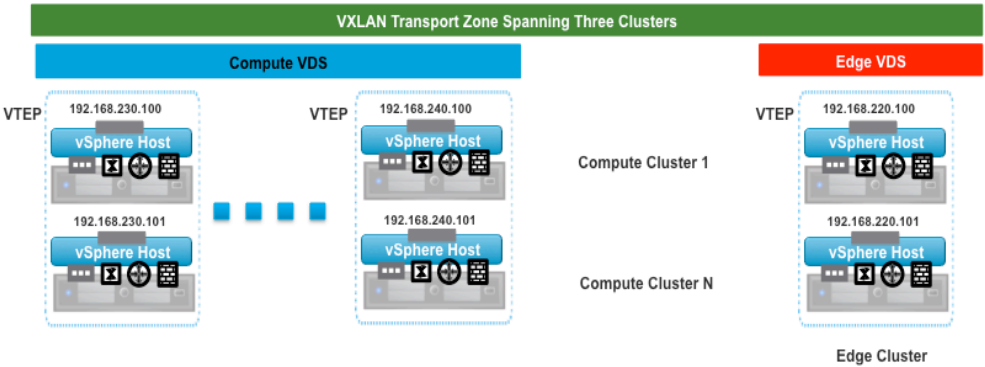
\includegraphics[width=0.8\textwidth]{imaxes/conceptosPrevios/transportZoneSpan.png}
  \caption{VXLAN extendida sobre varios vDS, comunica varios cluster.}
  \label{fig:trasnportZoneSpan}
\end{figure}
\FloatBarrier

El uso de VXLAN es clave para separar la red física de la red virtual porque permite la creación de un mayor número de VLANs en el SDDC, ya que no se configuran directamente sobre los dispositivos de red, además, aportan más flexibilidad a la hora de administrar la red física, simplifica y mejora la escalabilidad de la red, y hace posible la implementación de servicios de red a través de software con VMware NSX. La cantidad de VXLAN que se deben configurar en un SDDC depende del modelo utilizado, en el modelo consolidado se define una única VXLAN, mientras que en el modelo estándar se recomienda configurar una VXLAN que alcance todos los \textit{virtual infrastructure domains} de todas las \textit{regions} (en caso de que halla más de una), una VXLAN a través de todos los \textit{virtual infrastructure domains} de una \textit{region} y otra VXLAN a través de todos los \textit{management domains} existentes, para así permitir el aprovisionamiento de recursos de red bajo demanda, establecer políticas en varias instancias de vCenter Server y permitir la migración de máquinas virtuales entre \textit{regions}. A continuación se explica el funcionamiento de una VXLAN y los elementos que intervienen:\\

\indent    Cuando un host ESXi envía un \textit{frame} a otro host ESXi, utilizan el protocolo VXLAN. Cuando el \textit{frame} sale de la máquina virtual origen, este pasa por el VTEP del host, que lo encapsula con varias cabeceras y lo transmite a la red. El \textit{frame} orginial se trata de un paquete Ethernet de capa 2, al que el VTEP le añade una cabecera VXLAN con el identificador VNI de la VXLAN a la que pertenece el \textit{frame}, una cabecera UDP que indica los puertos origen y destino en los VTEP que realizan la comunicación, una cabecera IP que contiene las direcciones IP del VTEP origen y del VTEP destino, y una cabecera Ethernet cabeceras que son la cabecera VXLAN, la cabecera IP, la cabecera UDP y una cabecera Ethernet que indica las direcciones MAC origen y destino de los respectivos VTEP\footnote{Puede que se indique como VTEP de destino la dirección IP del \textit{gateway} de la red, si el destinatario se encuentra en otra red física.} que realizan la comunicación [Fig. \ref{fig:frameVXLAN}]. La cabecera Ethernet original contiene las dirección MAC de la máquina virtual origen y la MAC de la máquina virtual destino.

\begin{figure}[h!]
  \centering
  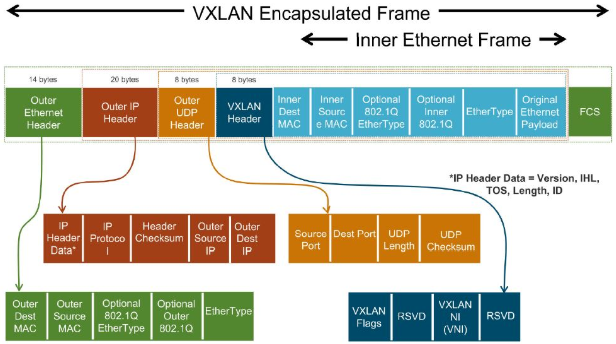
\includegraphics[width=0.8\textwidth]{imaxes/conceptosPrevios/frameVXLANv2.png}
  \caption{Cabeceras de un frame cuando se usa VXLAN.}
  \label{fig:frameVXLAN}
\end{figure}
\FloatBarrier

La información sobre VTEP existentes, la relación entre direcciones MAC de máquinas virtuales y dirección IP de VTEP, y relación entre direcciones MAC de máquinas virtuales y su IP, la poseen las instancias de NSX Controller en tres tablas: 
    \begin{itemize}
        \item \textit{VTEP Table}, relación entre un VTEP y la VXLAN que tiene acceso: VNI (ID del segmento), IP (dirección IP del VTEP), Segment (dirección IP del segmento), MAC (dirección MAC de la NIC física donde está configurado el VTEP).
        \item \textit{MAC Table}, relación entre la dirección MAC de una máquina virtual y el VTEP que le da acceso: VNI (ID del segmento), MAC (dirección MAC de la máquina virtual accesible por la VTEP-IP), VTEP-IP (dirección IP del VTEP que da acceso a la máquina virtual de la MAC indicada).
        \item \textit{ARP Table}, relación entre la dirección MAC y la dirección IP de una máquina virtual: VNI (ID del segmento), IP (dirección IP de la máquina virtual), MAC (dirección MAC de la máquina virtual).
    \end{itemize}
Estas tablas permiten reducir la cantidad de tráfico en la red ya que las máquinas virtuales y dispositivos de enrutamiento ya no requieren enviar tráfico Broadcast para obtenerla.
La comunicación directa entre máquinas virtuales situadas en distintos hosts ESXi se realiza con tráfico Unicast entre sus respectivos VTEP, pero una máquina virtual también puede enviar tráfico dirigido a todas las máquinas virtuales que pertenecen a su mismo Logical Switch, es decir, a las máquinas de la misma \textit{trasnport zone}, pero pueden situarse en segmentos de red físicos distintos. Este tipo de tráfico puede ser Multicast, Unknown Unicast y Broadcast (BUM), y en VMware NSX se puede gestionar con tres modos de replicación distintos\footnote{Al configurar un Logical Switch se elige uno de los modos.}, modo Multicast, modo Unicast y modo Híbrido.
    \begin{itemize}
        \item \textbf{Modo Multicast}: requiere que en la red física se haya configurado una IP multicast para cada VXLAN (es decir, Logical Switch), y el protocolo IGMP Snooping en los switches físicos para crear grupos multicast y que el tráfico sea más eficiente, esto habilita multicast entre los VTEP de la misma subred que el emisor. Para transmitir este tráfico a VTEPs situados en otros segmentos de red, se debe configurar el protocolo PIM para poder enrutarlo con los dispositivos de capa 3 físicos. Esta configuración no permite desacoplar la red lógica de la red física.\\
        Se puede establecer un grupo multicast por cada VXLAN, esto implica que un host solo recibirá tráfico si tiene al menos una máquina virtual en el grupo, pero requiere configurar muchos grupos. Otra opción es crear un grupo multicast para todas las VXLAN, se necesitan menos direcciones IP pero se genera más tráfico en la red.
    \begin{figure}[h!]
    \centering
    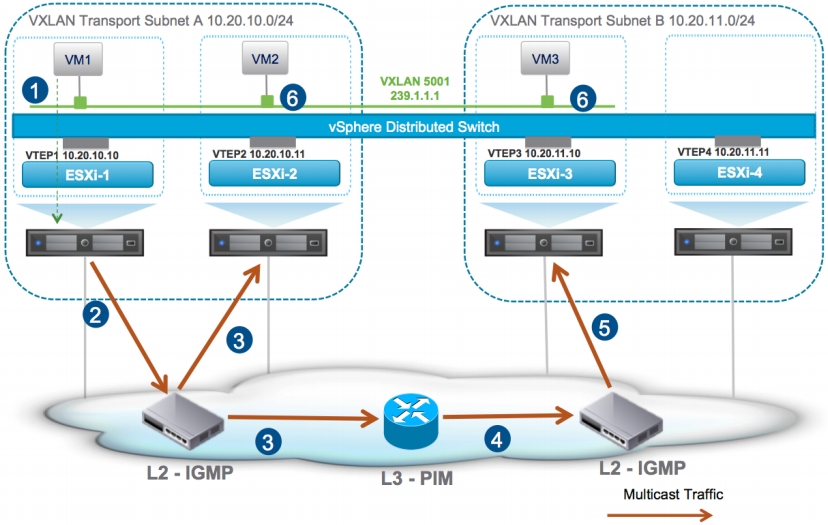
\includegraphics[width=0.5\textwidth]{imaxes/conceptosPrevios/MulticastSeqBUM.png}  \caption{Replicación del tráfico BUM en el modo Multicast}
    \label{fig:modoMulticast}
    \end{figure}
    \FloatBarrier
        \item \textbf{Modo Unicast}: no requiere ninguna configuración específica en la capa física y está gestionado por VMware NSX. Se crea un grupo con los VTEP situados en el mismo segmento de red, dentro de cada grupo se selecciona un host ESXi para el rol de \textit{Unicast Tunnel End Point} (UTEP), encargado de recibir el tráfico BUM que procede de otros segmentos de red para reenviarlo por su segmento pero solo a los hosts con al menos una máquina virtual. El host ESXi emisor utiliza la tabla VTEP para comprobar que VTEPs están situados en una VXLAN y así poder dirigir el tráfico BUM correspondiente.\\
        Este modo es útil en entornos pequeños donde no hay mucho tráfico y cada segmento de red tiene pocos VTEP.
    \begin{figure}[h!]
    \centering
    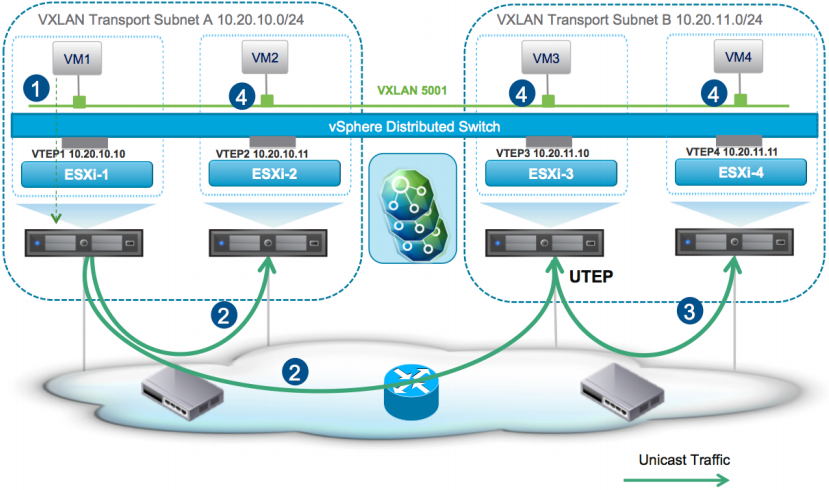
\includegraphics[width=0.5\textwidth]{imaxes/conceptosPrevios/UnicastMode.png}
    \caption{Replicación del tráfico BUM en el modo Unicast}
    \label{fig:modoUnicast}
    \end{figure}
    \FloatBarrier
        \item \textbf{Modo Híbrido}: combina el modo Unicast y el modo Multicast. El tráfico dirigido a las máquinas virtuales situadas en el mismo segmento de red se transmite usando Multicast, por lo que se requiere tener el protocolo IGMP configurado en los dispositivos físicos de capa 2, se recomienda establecer una dirección Multicast por cada VXLAN. El tráfico se replica a los hosts ESXi que forman parte del grupo. Cuando el tráfico va dirigido a máquinas virtuales situadas en hosts en distinto segmento de red, se transmite utilizando Unicast, como en ese modo, se forma un grupo con los hosts de cada segmento y de cada grupo se elige un host con el rol de \textit{Multicast Tunnel EndPoint} (MTEP). Así, el host que origina el tráfico BUM lo transmite al MTEP correspondiente, el cual se encarga de replicar ese tráfico por su segmento de red. La replicación del tráfico entre segmentos es gestionada por las instancias de NSX Controller.\\
        Este modo de replicación permite desplegar NSX en entornos grandes gracias a que el tráfico Multicast y Unicast se pueden escalar facilmente, el primero se reduce a cada segmento de red y la transmisión del segundo en la capa 3 está gestionado por VMware NSX sin necesidad de configurar los dispositivos físicos.
    \begin{figure}[h!]
        \centering
        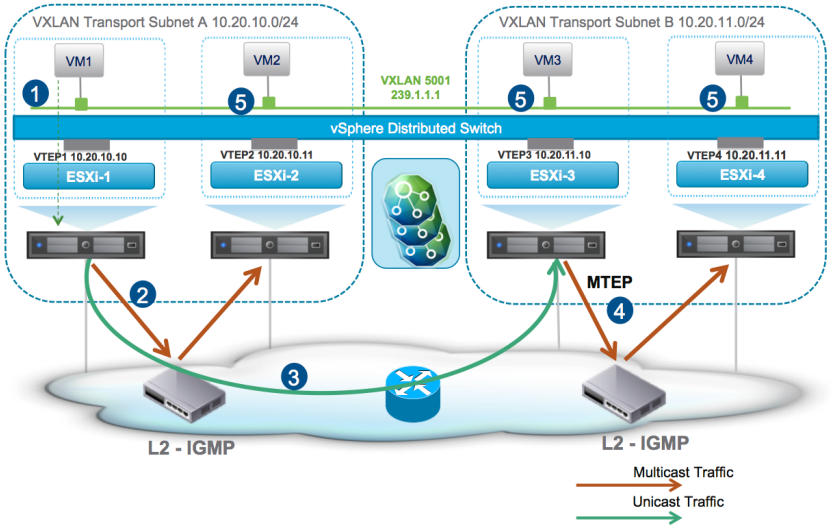
\includegraphics[width=0.5\textwidth]{imaxes/conceptosPrevios/hibrydMode.png}
        \caption{Replicación del tráfico BUM en el modo Híbrido}
        \label{fig:modoHibrido}
    \end{figure}
    \FloatBarrier
    \end{itemize}

 El enrutamiento del tráfico está gestionado por dos componentes Distributed Logical Router (DLR) y NSX Edge Services Gateway (ESG). Un mismo DLR se extiende por varios hosts ESXi para enrutar el tráfico entre VXLANs, también mantiene una conexión con las instancias de ESG para transmitir el tráfico que se dirige a redes externas, esa conexión se denomina \textit{transit network} y está getionada por un Logical Switch. Cada DLR tiene su propio Logical Router Control para intercambiar las rutas disponibles con las instancias de ESG, posteriormente, son las instancias de NSX Controller las que transmiten esta información al DLR distribuido en los hosts ESXi. Las interfaces lógicas del DLR conectan con cada Logical Switch, cada interfaz tiene una dirección IP que representa el \textit{gateway} del segmento de red al que esté conectada [Fig. \ref{fig:logicalRoutingCompo} y \ref{fig:redLogicaOne}]. Estos dispositivos utilizan enrutamiento dinámico (protocolos OSPF o BGP).
 
 \begin{figure}[h!]
  \centering
  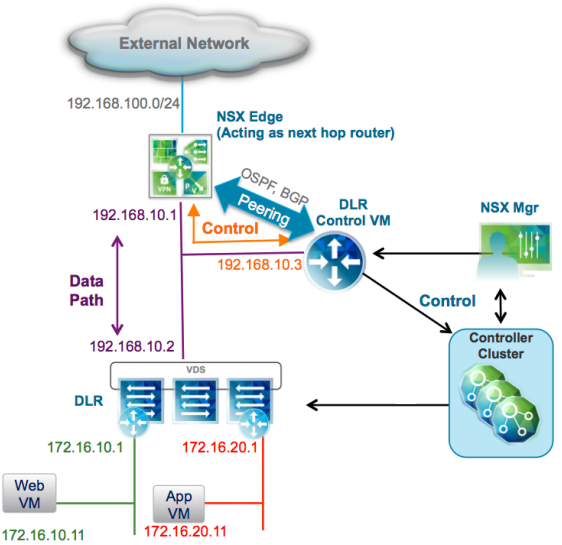
\includegraphics[width=0.4\textwidth]{imaxes/conceptosPrevios/LogicalRoutingComponents.png}
  \caption{Componentes de la red virtual que intervienen en el enrutamiento del tráfico.}
  \label{fig:logicalRoutingCompo}
\end{figure}
\FloatBarrier

\begin{figure}[h!]
  \centering
  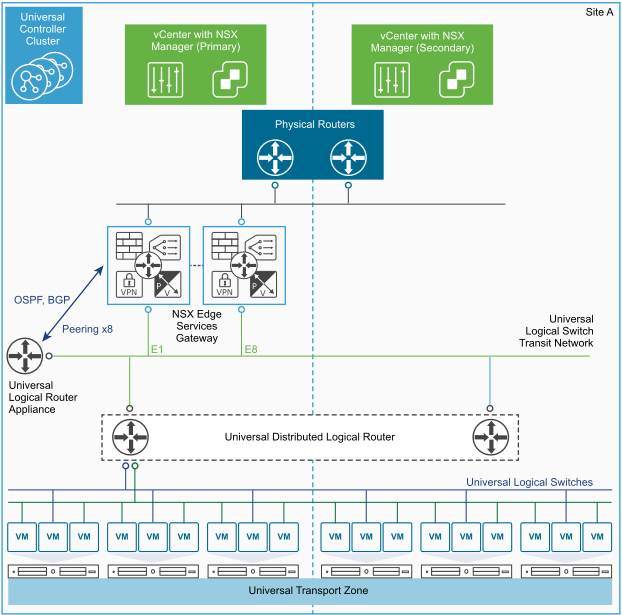
\includegraphics[width=0.5\textwidth]{imaxes/conceptosPrevios/redlogCF.png}
  \caption{Red lógica formada en un SDDC con dos clusters.}
  \label{fig:redLogicaOne}
\end{figure}
\FloatBarrier
 
 En el SDDC deben existir, al menos, dos intancias de ESG aunque se pueden desplegar hasta 8 instancias. En el modelo consolidado se debe tener un único UDLR para que las rutas entre hosts ESXi sean más cortas, debe existir un Logical Switch que forme la \textit{transit zone}. En el modelo estándar debe existir un UDLR extendido por todos los \textit{Management Cluster} (si hay varias \textit{Regions}), un UDLR extendido por el \textit{Shared Edge and Compute Cluster} y el resto de \textit{Compute Clusters} en cada \textit{Region}, y un DLR extendido por todos los clusters de una misma región.En el modelo estándar existen dos tipos de \textit{transit zones}, una entre el UDLR que atraviesa todas las \textit{Regions} y cada instancia de ESG, y otra que conecta el DLR propio de cada \textit{Region} y sus instancias de ESG. 
\\
Algunos componentes de VMware Cloud Foundation se deben desplegar en una VXLAN dedicada para proporcionar recuperación ante fallos en caso de que parte del SDDC deje de funcionar. Entre otros componentes (solo vamos a tratar aquellos que son obligatorios), VMware vRealize Log Insight se debe desplegar en una red de este tipo, llamada \textit{Application Virtual Network} (AVN). En entornos con varias \textit{Regions} se crea una \textit{transport zone} que se extiende por todo el SDDC y una \textit{transport zone} adicional en cada \textit{Region}, la primera proporciona recuperación ante fallos a través de todo el SDDC a los componentes que lo requieran, y la segunda solo a través de una \textit{Region}, sin necesidad de reconfigurar direcciones IP o DNS. VMware vRealize Log Insight se debe desplegar en una VXLAN por cada \textit{Region}.
\\
El acceso a una AVN se realiza a través de las instancias de ESG desplegadas en el entorno, estas se conectan a un UDLR que gestiona el tráfico de la s máquinas virtuales que tiene conectadas. El enrutamiento debe ser dinámico con BGP y las instancias de ESG proporcionan protegen y balacean la carga de trabajo con los servicios de VMware NSX Firewall y Load Balancing [Fig. \ref{fig:avnConsolidated}].\\
**VERIFICAR LO DEL LOAD BALANCING en el despliegue. ¿solo para las que son cross-region o tambien en las de una sola region**\\
\begin{figure}[h!]
  \centering
  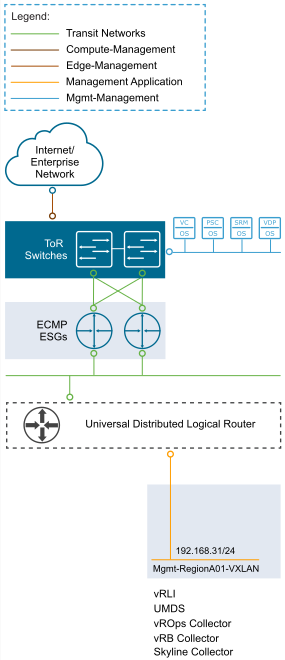
\includegraphics[width=0.25\textwidth]{imaxes/conceptosPrevios/AVNConsolidated.png}
  \caption{AVN en el modelo consolidado}
  \label{fig:avnConsolidated}
\end{figure}
\FloatBarrier



\iffalse
\begin{figure}[h!]
  \centering
  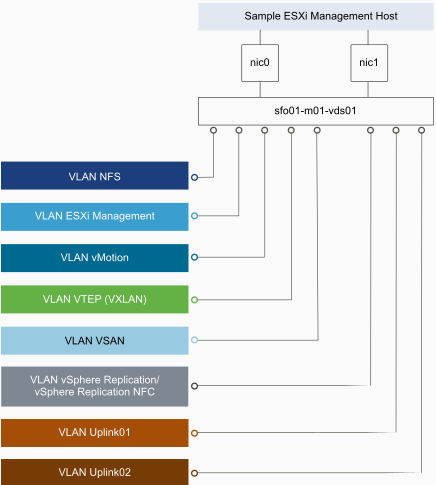
\includegraphics[width=0.65\textwidth]{imaxes/conceptosPrevios/redesVDSCluster.png}
  \caption{Redes virtuales que se utilizan en en la infraestructura para cada componente.}
  \label{fig:redesVirtuales}
\end{figure}
\FloatBarrier
Este utiliza los componentes vCenter Server, NSX Manager, NSX Controllers y NSX Logical Switch para establecer comunicaciones y aislar los distintos tipos de tráfico [Fig. \ref{fig:planosNSX}]. Estos componentes \underline{actúan en diferentes planos} de la red:



\begin{itemize}
    \item \textbf{Plano de Datos}: esta capa gestiona la transmisión del tráfico entre los componentes del SDDC. En este plano actúan NSX Logical Switches segregando los tipos de datos, y el enrutamiento y firewall distribuído de NSX. Se transmite a través de una red física dedicada al transporte.
    \item \textbf{Plano de Control}: aquí se gestionan los mensajes de control que se usan para la configuración de los dispositivos de NSX como switches, routers y firewalls en cada host ESXi. Se distribuye en redes físicas de forma segura usando VLANs para aislarlo del plano de datos.
    \item \textbf{Plano de gestión}: aquí se gestiona el tráfico dedicado a la administración de los recursos como puede ser la creación y eliminación de máquinas virtuales. Está controlado por vCenter Server y NSX Manager.
\end{itemize}
\begin{figure}[h!]
  \centering
  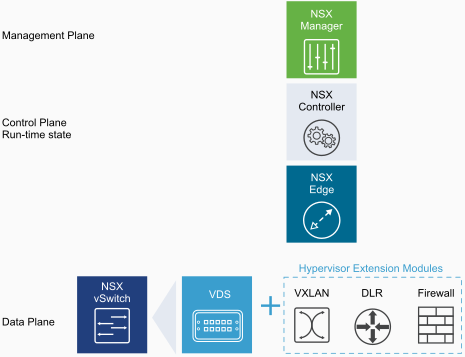
\includegraphics[width=0.65\textwidth]{imaxes/conceptosPrevios/planosNSX.png}
  \caption{Como se estructuran las componentes de VMware NSX for vSphere}
  \label{fig:planosNSX}
\end{figure}
\FloatBarrier
Adicionalmente, VMware NSX incluye diversos servicios que suponen una abstracción lógica de dispositivos físicos de red y que VMware Cloud Foundation utiliza para formar su infraestructura virtual. Estos \underline{servicios son los siguientes}\cite{componentesNSX,nsxCompDesign}:
\begin{itemize}
    \item \textbf{Logical Switches}: permite crear segmentos abstractos que representan dominios de broadcasting donde se colocan determinadas máquinas virtuales. Su tráfico tiene asignado una única VLAN y están mapeados en todos los hosts lo cual simplifica la movilidad de las máquinas virtuales entre los hosts.
    \item \textbf{Universal Distributed Logical Router} (UDLR): realiza las funciones de enrutamiento entre máquinas virtuales y entre \textit{portgroups} de una VXLAN [Pal. \ref{itm:vxlan}]. Se controlan desde una máquina virtual. 
    %y utilizan protocolos de enrutamiento dinámico como BGP y OSPF.
    \item \textbf{Designated Instance}: host ESXi encargado de resolver las solicitudes del protocolo ARP. Es elegido por NSX Controller que escoge un host por cada VLAN existente.
    \item \textbf{Edge Services Gateway} (ESG): también llamado NSX Edge, es el encargado de proveer conectividad a través de la infraestructura física para que los componentes se puedan conectar a redes externas u otras redes del la infraestructura. También aporta firewall de perímetro, balanceo de carga y SSL-VPN.
    \item \textbf{Logical Firewall}: provee mecanismos de seguridad que se asemejan a las funciones de los firewalls físicos pero con la ventaja de que están virtualizados, lo cual hace que su configuración sea más flexible. Trabaja al nivel de puertos \textit{vmkernel} y máquinas virtuales.
    \item \textbf{Logical Load Balancer}: distribuye el tráfico entre los servidores para que el uso de recursos sea el óptimo.
    \item \textbf{VXLAN Tunnel Endpoint} (VTEP): punto donde se encapsula el tráfico de VXLAN en paquetes UDP. Se ubican en los puertos \textit{vmkernel} de un vSphere Distributed Switch.
\end{itemize}
\fi

\iffalse
\subsubsection{Almacenamiento Virtual}
VMware vSAN forma único \textit{datastore} con todos los dispositivos de almacenamiento que se encuentran en la infraestructura permitiendo establecer políticas y gestionar esos recursos de forma más simple. Para que funcione correctamente es necesario \underline{configurar una red para VMware vSAN} teniendo en cuenta los siguientes aspectos:
\begin{itemize}
    \item El uso de vSpehere Distributed Switches genera mejor rendimiento.
    \item Se recomienda el uso de paquetes tipo \textit{jumbo frames}.
    \item Asignar una VLAN al tráfico de cada cluster de VMware vSAN.
    \item Si se implementa en un SDDC con dos localizaciones, es necesario establecer un host \textit{witness}.
\end{itemize}
Al establecer el tamaño y capacidad de este cluster hay que tener en cuenta que cuantos más hosts ESXi se incluyan, mayor tolerancia a fallos se tendrá y mejor se podrán repartir los grupos de discos entre todos los hosts. Debe haber un balance entre el hardware y la capacidad requerida.
\end{subsection}

\fi



\begin{subsection}{Operaciones de la Arquitectura\cite{CFopermanagement}}
En este apartado se define como se gestionan en VMware Cloud Foundation las tareas de administración de todas las partes de la infraestructura. Estas tareas se agrupan en la gestión del ciclo de vida y la recopilación de información sobre el estado de cada componente existente.

\subsubsection{Gestión del Ciclo de Vida}
Elementos que se encargan de administrar el ciclo de vida de los componentes:
\begin{itemize}
    \item \textbf{vSphere Update Manager}: por cada instancia de VMware vCenter Server se despliega una instancia de vSphere Update Manager. Este componente utiliza el servicio \textit{Update Manager Download Service} (UMDS) para obtener las actualizaciones de la red externa al SDDC, el cual se despliega en una red AVN [Fig. \ref{fig:avnConsolidated}], permitiendo limitar el acceso a Internet de vSphere Update Manager y reduciendo el número de descargas ya que un UMDS se comparte entre varias instancias de VMware vCenter Server. Se crea una instancia de UMDS por cada \textit{region} existente [Fig. \ref{fig:UpdateManagerArc}].
    \begin{figure}[h!]
        \centering
        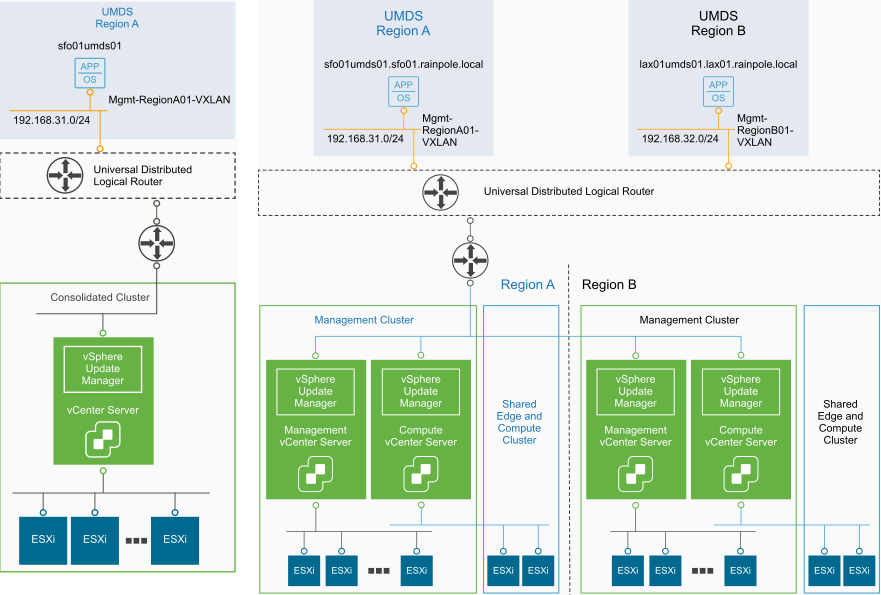
\includegraphics[width=0.5\textwidth]{imaxes/conceptosPrevios/UpdateManagerArch.png}
        \caption{Diseño de vSphere Update Manager en el modelo consolidado (izquierda) y en el modelo estándar (derecha)}
        \label{fig:UpdateManagerArc}
    \end{figure}
    \FloatBarrier
    
    \item \textbf{vRealize Suite Licfecycle Manager}: componente utilizado para desplegar, actualizar y configurar, de forma automatizada, los productos vRealize Operations, vRealize Log Insight, vRealize Automation y vRealize Business Cloud. De este componente se despliega una única instancia en una AVN accesible desde cada \textit{region} por todas las instancias de VMware vCenter Server. Se debe registrar su nombre de dominio en el servidor DNS para hacerla accesible.
    
    \iffalse
    y se puede elegir entre dos modelos de despliegue, uno en el que se usa una máquina virtual denominada  que se encarga de descargar los archivos requeridos por vSphere Update Manager mientras este se encuentra en un entorno aislado [Fig. \ref{fig:updateManager}], y otro donde es la instancia de vSphere Update Manager la que realiza la descarga de los ficheros. La primera opción incrementa la seguridad y permite compartir estos archivos entre distintas instancias de vSphere Update Manager.\\
    Una vez desplegado se pueden establecer diferentes configuraciones a nivel de host, máquina virtual y cluster, para que durante la instalación de actualizaciones el servicio del SDDC continúe operativo y evitar la pérdida de información y errores en los recursos.
    \begin{figure}[h!]
  \centering
  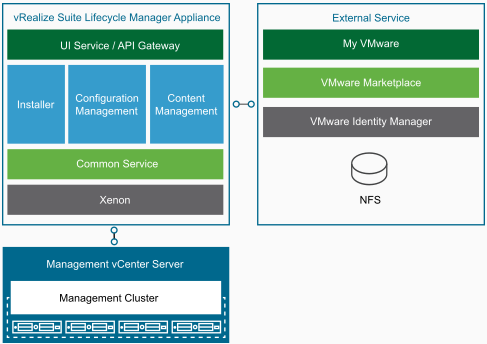
\includegraphics[width=0.8\textwidth]{imaxes/conceptosPrevios/vRealizeUpdateArchLifeCyle.png}
  \caption{Estructura de la gestión del ciclo de vida con vRealize Suite Lifecycle Manager.}
  \label{fig:vrealizeUpdateManager}
\end{figure}
\FloatBarrier
    \fi


\end{itemize}




\subsubsection{Gestión de Logs}
En VMware Cloud Foundation el producto vRealize Log Insight provee gestión y análisis de los logs de la infraestructura. Este componente resgistra los logs, alarmas y eventos de Platform Services Controller, instancias de VMware vCenter Server, de los hosts ESXi, componentes de VMware NSX, vRealize Suite Lifecycle Manager y componentes de vRealize Automation, utilizando el protocolo \textit{syslog} para su obtención. En el modelo consolidado se recomienda desplegar vRealize Log Insight en tamaño reducido, es decir, un solo nodo \textit{master} que gestiona los logs de todos los componentes, pero también se pueden desplegar otros nodos \textit{worker}. Para el modelo estándar se deben desplegar al menos tres nodos por cada \textit{region}, uno \textit{master} y dos \textit{worker}, y el uso de Load Balancer proporciona tolerancia a fallos en caso de que falle uno de los nodos. En ambos modelos los nodos se despliegan en una AVN que solo se extiende por una \textit{region} [Fig. \ref{fig:redLogIsight}], también se deben configurar la dirección IP y nombre de dominio de cada nodo en el servicio DNS.
    \begin{figure}[h!]
  \centering
  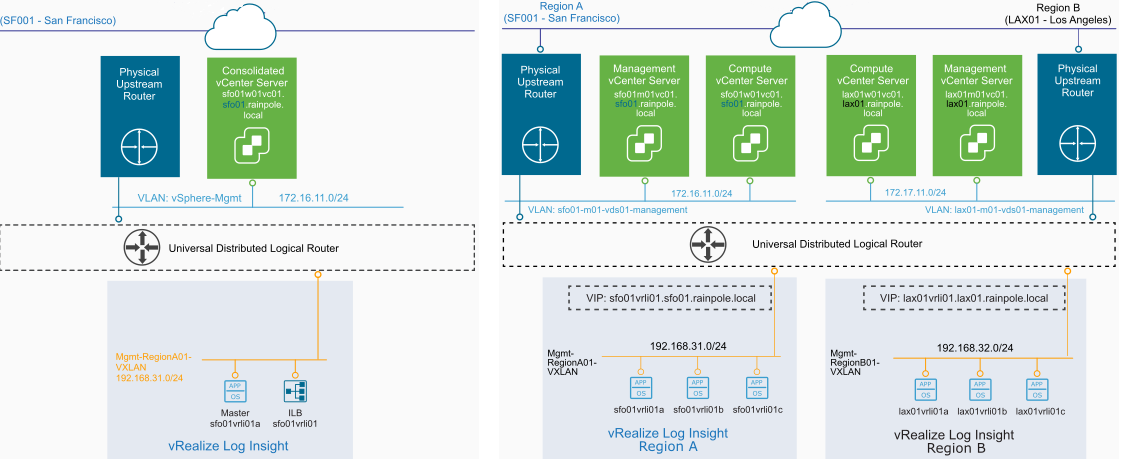
\includegraphics[width=0.7\textwidth]{imaxes/conceptosPrevios/networkLogInsight.png}
  \caption{Localización de vRealize Log Insight en el modelo consolidado (izquierda) y en el modelo estándar (derecha)}
  \label{fig:redLogIsight}
\end{figure}
\FloatBarrier
\end{subsection}
